\begin{pastexam}[label={px:ncku-111-cce-ds-02}]{成大電通所 111 學年度 第 2 題}
（問答）

(10 \textbf{pts}) Biconnected components
\begin{enumerate}[label=\alph*.]
\item (2 \textbf{pts}) Please give the definition of a back edge ($u$, $v$) in an undirected
graph.
\item (6 \textbf{pts}) Describe the two rules to find the articulation points and explain why
they are correct.
\item (2 \textbf{pts}) Show all biconnected components in the right graph.
\end{enumerate}
\begin{center}
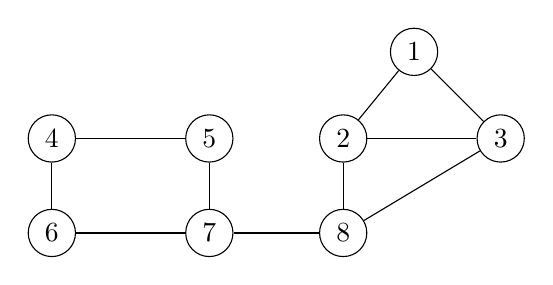
\begin{tikzpicture}[v/.style={circle,draw,inner sep=1pt,minimum size=6mm}]
\node[v] (4) at (0,1.2) {4}; \node[v] (5) at (2,1.2) {5};
\node[v] (6) at (0,0) {6}; \node[v] (7) at (2,0) {7}; \node[v] (8) at (3.7,0) {8};
\node[v] (2) at (3.7,1.2) {2}; \node[v] (3) at (5.7,1.2) {3}; \node[v] (1) at (4.6,2.3) {1};
\foreach \a/\b in {4/5,4/6,5/7,6/7,7/8,1/2,1/3,2/3,2/8,3/8} \draw (\a) -- (\b);
\end{tikzpicture}
\end{center}
\end{pastexam}

\begin{pastsoln}
答案：(a) 不在 DFS 樹上、連到祖先的邊；(b) 根有兩個以上子節點／非根 $u$ 有子節點 $w$ 使
$\mathit{low}(w) \ge \mathit{dfn}(u)$；(c) 雙連通元件是 $\{4, 5, 6, 7\}$、$\{7, 8\}$、
$\{1, 2, 3, 8\}$，割點是 $7$ 和 $8$。

\textbf{(a) 後向邊。} 對無向圖做 DFS，得到 DFS 樹（森林）。 一條邊 $(u, v)$ 如果\textbf{不是}
樹邊，而且 $v$ 是 $u$ 的祖先（DFS 時從 $u$ 看到已經拜訪過、還沒結束的 $v$，而且 $v$ 不是 $u$
的父節點），就叫後向邊（back edge）。 無向圖的 DFS 中，每一條非樹邊都連接祖先和後代，所以非樹邊
全都是後向邊（資結書第~21.5~節定理~21.8）。

\textbf{(b) 判斷割點的兩條規則}（資結書第~23.5~節定理~23.8、23.9）。 先定義
$\mathit{dfn}(u)$ 是 $u$ 在 DFS 中被拜訪的順序，
\[
\mathit{low}(u) = \min\bigl\{\mathit{dfn}(u),\ \min\{\mathit{low}(w) : w \text{ 是 } u
\text{ 的子節點}\},\ \min\{\mathit{dfn}(v) : (u, v) \text{ 是後向邊}\}\bigr\},
\]
也就是從 $u$ 往下沿樹邊走、最後最多走一條後向邊，能到達的最小 $\mathit{dfn}$。
\begin{enumerate}[label=\arabic*.]
\item \textbf{根}是割點，若且唯若它在 DFS 樹上有兩個以上子節點。
\item \textbf{非根}的 $u$ 是割點，若且唯若它有一個子節點 $w$ 滿足
$\mathit{low}(w) \ge \mathit{dfn}(u)$。
\end{enumerate}

為什麼對：
\begin{itemize}
\item 規則 1：根的兩棵不同子樹之間沒有邊。 無向 DFS 沒有交叉邊，子樹之間若有邊，DFS 會從第一棵
子樹直接走過去，第二棵就不會是另一個子節點。 所以根有兩個以上子節點時，拿掉根，子樹之間就斷了；
只有一個子節點時，拿掉根剩下的就是一棵完整的子樹，仍然連通。
\item 規則 2：拿掉非根的 $u$ 之後，$u$ 的子樹 $T_w$ 要和外面（$u$ 的祖先那邊）連得上，只能靠
$T_w$ 裡某個點的後向邊連到 $u$ 的\textbf{嚴格}祖先（無向 DFS 沒有交叉邊）。 嚴格祖先的
$\mathit{dfn}$ 都比 $\mathit{dfn}(u)$ 小，所以「$T_w$ 連得出去」等價於
$\mathit{low}(w) < \mathit{dfn}(u)$。 有某個子節點 $w$ 的 $\mathit{low}(w) \ge
\mathit{dfn}(u)$，拿掉 $u$ 後 $T_w$ 就和祖先那邊分開，$u$ 是割點；反過來，每個子節點都
$\mathit{low}(w) < \mathit{dfn}(u)$ 時，每棵子樹都接得回祖先，圖仍然連通（非根的 $u$ 一定有
父節點，祖先那邊不是空的）。
\end{itemize}

\textbf{(c) 雙連通元件。} 從頂點 $1$ 開始 DFS，鄰點照編號由小到大。 DFS 樹剛好是一條路徑
$1 - 2 - 3 - 8 - 7 - 5 - 4 - 6$，後向邊是 $(3, 1)$、$(8, 2)$、$(6, 7)$：
\begin{center}
\begin{tabular}{c*{8}{c}}
\toprule
頂點 & 1 & 2 & 3 & 8 & 7 & 5 & 4 & 6 \\
\midrule
$\mathit{dfn}$ & 1 & 2 & 3 & 4 & 5 & 6 & 7 & 8 \\
$\mathit{low}$ & 1 & 1 & 1 & 2 & 5 & 5 & 5 & 5 \\
\bottomrule
\end{tabular}
\end{center}
$\mathit{low}$ 由下往上算：$6$ 有後向邊到 $7$，$\mathit{low}(6) = 5$，往上傳給 $4, 5, 7$；$8$ 有
後向邊到 $2$，$\mathit{low}(8) = 2$；$3$ 有後向邊到 $1$，$\mathit{low}(3) = 1$，傳給 $2$。

套規則：根 $1$ 只有一個子節點，不是割點。 $8$ 的子節點 $7$：$\mathit{low}(7) = 5 \ge
\mathit{dfn}(8) = 4$，$8$ 是割點。 $7$ 的子節點 $5$：$\mathit{low}(5) = 5 \ge \mathit{dfn}(7) = 5$，
$7$ 是割點。 其餘：$2$（子 $3$，$1 < 2$）、$3$（子 $8$，$2 < 3$）、$5$（子 $4$，$5 < 6$）、$4$（子
$6$，$5 < 7$）都不是。 割點是 $\{7, 8\}$。

在割點處切開，雙連通元件（極大的、沒有割點的連通子圖，資結書第~23.6~節）有三個：
\begin{itemize}
\item $\{4, 5, 6, 7\}$，邊 $(4,5), (4,6), (5,7), (6,7)$：一個四邊形環。
\item $\{7, 8\}$，邊 $(7,8)$：一座橋，自己是一個元件。
\item $\{1, 2, 3, 8\}$，邊 $(1,2), (1,3), (2,3), (2,8), (3,8)$：兩個三角形共用邊 $(2,3)$。
\end{itemize}
$10$ 條邊恰好分在三個元件裡（$4 + 1 + 5$），元件之間只在割點 $7$、$8$ 相接。
\end{pastsoln}
